%!TEX root = ../thesis.tex
\label{part:DRIE}







% \part{asdf}{dfgs}
\part{Deep-reactive ion etched resonators\protect\blfootnote{This experiment has been published in Applied Physics Letters \textbf{106} 18 (2015).}}
\label{chapter:Resonators}

\chapter{Theory}
  \label{ch:theory}

  \section{Coplanar waveguide}
    \captionsetup[subfigure]{position=top}
    \begin{figure}[h]
      \begin{subfigure}{.49\textwidth}
        \begin{center}
            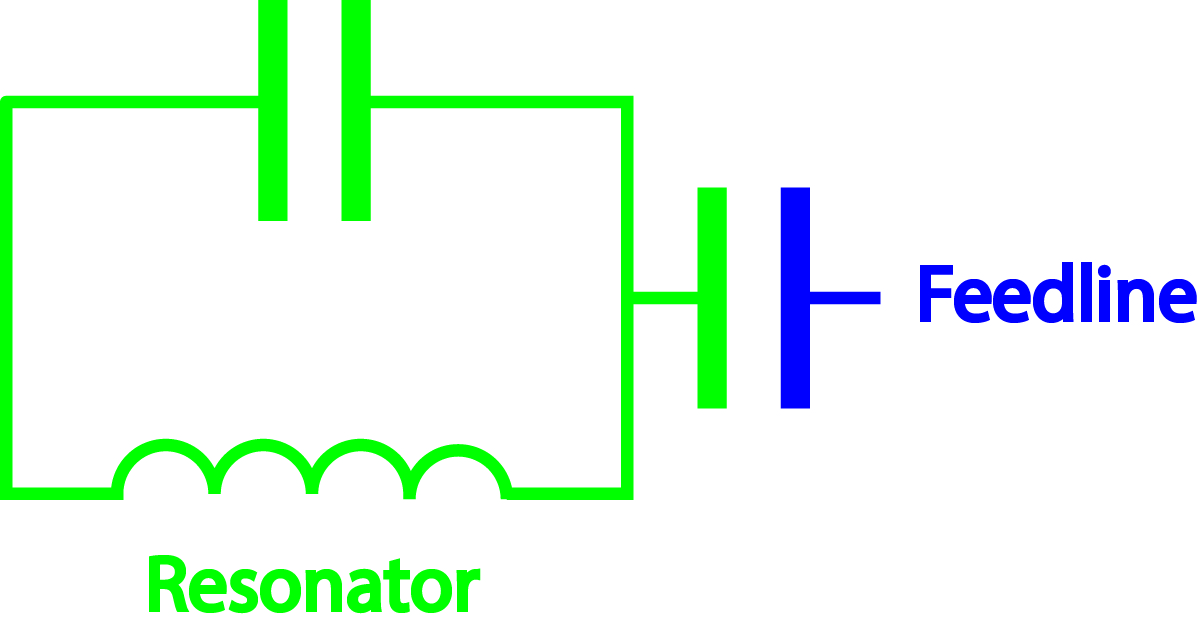
\includegraphics[width=.8\textwidth]{Figures/DRIE/resonator schematic joined.jpg}
        \end{center}
        \caption{ }
        \label{fig:CPW schematic}
      \end{subfigure}
      ~
      \begin{subfigure}{.49\textwidth}
        \begin{center}
            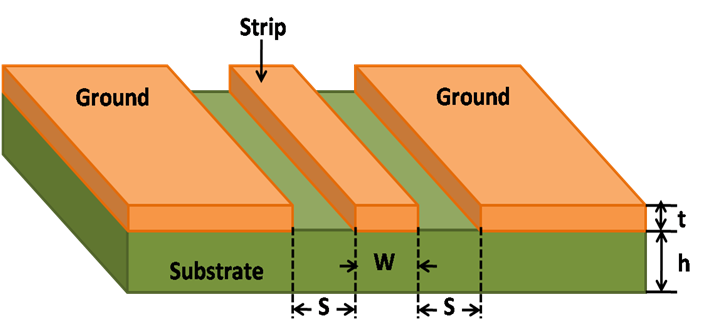
\includegraphics[width=.8\textwidth]{Figures/DRIE/CPW.png}
        \end{center}
        \caption{ }
        \label{fig:CPW intersection}
      \end{subfigure}
      \caption{\textbf{(a)} A resonator circuit diagram, including capacitive coupling to a feedline. \textbf{(b)} Cross-section on a CPW resonator. For a typical resonator $w=\SIm{12}{\micro \meter}$, $s=\SIm{5}{\micro \meter}$, $t=\SIm{200}{\nano \meter}$, and $h=\SIm{525}{\micro \meter}$.}
      \label{fig:CPW}
    \end{figure}
    \captionsetup[subfigure]{position=top}

    % \begin{wrapfigure}{r}{0.4\textwidth}
    %     \begin{center}
    %         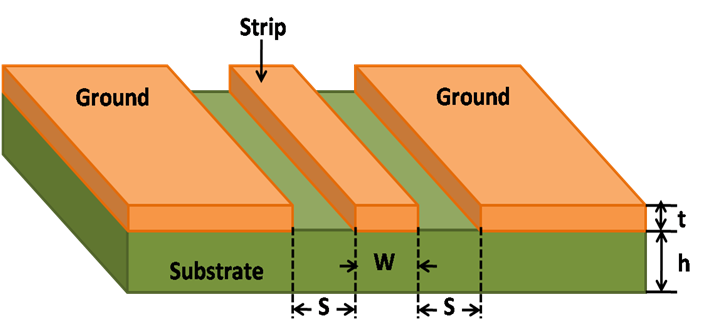
\includegraphics[width=\textwidth]{Figures/DRIE/CPW.png}
    %     \end{center}
    %     \caption{Schematic of a coplanar waveguide. For a typical resonator $w=\SIm{12}{\micro \meter}$, $s=\SIm{5}{\micro \meter}$, $t=\SIm{200}{\nano \meter}$, and $h=\SIm{525}{\micro \meter}$.}
    %     \label{fig:CPW}
    % \end{wrapfigure}

    Superconducting coplanar waveguides (CPW) microwave resonators have versatile applications. They are used in single-photon detectors~\cite{tanner2010enhanced}, quantum-limited Josephson parametric amplifiers~\cite{castellanos2008amplification}, and in the context of circuit QED are used for memory storage, readout, and as interconnects. Coplanar waveguides consist of a long central conducting strip, with on both sides a neighbouring ground. The center conductor of width $w$ is separated from the neighbouring grounds by a fixed gap $s$.

    For qubit readout one end is usually capacitively coupled to a feedline and has an open end, while the other end can either be open or shorted. This determines whether the current has a node or an anti-node at that end. In the case of a shorted end, current has an anti-node at that end, resulting in a quarter-wave resonator. This means that the wavelength of the fundamental mode fits a quarter times into the resonator. In the case of an open end, the current has a node at that end, resulting in a half-wave resonator.


  \section{Quality factor}
    \label{sec:Quality factor}
    % TODO
    % Find where it says that loss tangents can be added to each other
    % Include the fact that participation ratios are needed for adding quality factors of loss channels
    % Explain why one wants a quality factor that is as high as possible
    The quality of a resonator can be quantified by its quality factor. Generally speaking, the quality factor of a resonator determines the ratio between energy stored in a resonator and the energy dissipated from the resonator. For cQED resonators this corresponds to the rate at which photons leak out of the resonator. A high quality factor corresponds to a low dissipation rate.

    The quality factor can also be defined in two different ways \cite[pp.23-24]{Mazin}:

    \begin{equation}
        Q = \omega_r \tau_1 = \omega_r / \Delta \omega.
        \label{eqn:quality factor definition}
    \end{equation}
    Here, $\omega_r$ is the resonance frequency of the resonator, $\Delta \omega$ is the full width at half maximum, and $\tau_1$ is the decay time of the resonator. The decay time is the time after which the energy of a resonator is dissipated to $1/e$ of its original value.

    Photons can be lost through different loss channels. Each of these loss channels has a corresponding quality factor. One such loss channel is due to resonators being capacitively coupled to a feedline. The quality factor associated to this loss channel is known as the coupling quality factor $Q_c$, and depends on the amount of capacitive coupling between the resonator and the feedline. It can therefore be engineered to have a certain value, depending on the desired interaction between resonator and feedline.

    The other loss channels are usually unwanted, and therefore desired to be as low as possible. These individual channels are usually lumped together, resulting in a combined quality factor, known as the internal quality factor $Q_i$.

    The total quality factor of the resonator is known as the loaded quality factor $Q_l$. It is related to $Q_c$ and $Q_i$ through

    \begin{equation}
        \frac{1}{Q_l} = \frac{1}{Q_c} + \frac{1}{Q_i}.
        \label{eq:Q_l}
    \end{equation}
    It can be seen that if the difference between $Q_c$ and $Q_i$ is large, then the loaded quality factor $Q_l$ will be approximately equal to the minimum of the two.

    For a quarter-wave resonator the amplitude of transmission has a minimum $S_{21}^{min}$, given by \cite[p29]{Mazin}
    \begin{equation}
        S_{21}^{min} = \frac{Q_c}{Q_c + Q_i}.
        \label{eq:S21min}
    \end{equation}
    With knowledge of the resonant frequency $\omega_r$, the resonant width $\Delta \omega$, and the transmitted signal at resonance $S_{21}^{min}$, it is possible through Eqs.~\ref{eqn:quality factor definition} and \ref{eq:S21min} to determine both the coupling quality factor $Q_c$ and the internal quality factor $Q_i$. Note that as Eq.~\ref{eq:S21min} depends on the ratio of the two quality factors, to get an accurate estimate of both quality factors, they should have a comparable value.

    One reason why a high quality factor is important in the context of cQED is that a qubit can be coupled to a resonator. The resonator shapes the electromagnetic field seen by the qubit. This can either cause enhanced or diminished emission, and is known as the Purcell effect. If a qubit is in the excited state, its coupling to the resonator will result in relaxation of its state to the ground state. This can be quantified through its relaxation time $T_1^\text{Purcell}$, given by~\cite{Reed}

    \begin{equation}
      T_1^\text{Purcell} = \left(\left(\frac{g}{\Delta}\right)^2\kappa\right)^{-1},
      \label{eq:purcell T1}
    \end{equation}
    where $\kappa=\omega_r/Q_i$ is the cavity decay rate.

    The reason a high quality factor is important is because the Purcell relaxation time is proportional to the quality factor. The Purcell relaxation time $T_1^\text{Purcell}$ places an upper limit on the relaxation time $T_1$ of a qubit. If the qubit's relaxation time $T_1$ is close to this value, the qubit is said to be Purcell limited.

  \section{Losses}
    \label{sec:Losses}

      When a resonator is being driven at its resonance frequency, it is dynamically loaded with photons. When this external driving stops, the photons in the resonator leak out through different loss channels.

      One loss channel has already been discussed in section~\ref{sec:Quality factor}, namely through the coupling to the feedline. This loss channel is not unwanted, as the amount of coupling to the feedline determines how fast the resonator and feedline can interact with each other. The other loss channels, however, are unwanted, as they have no added benefit, and result in an irreversible loss of information. Some of the main sources of photon loss will be discussed in this section.

  \subsection{Causes of loss}

    \subsubsection{Two-level systems}
      \label{sec:TLS}

      Two-level systems (TLS) are systems which can be in a ground state or in an excited state. In some cases they can be useful. In fact a qubit itself is a TLS. In other cases, however, TLS can be a source of dissipation, such as in the case of dielectric loss~\cite{martinis2014ucsb}. Study suggests that in cQED, most TLS reside in a thin layer at the metal-substrate interface and the substrate-air interface~\cite{wenner2011surface}.

      Energy dissipation due to dielectric loss can be modeled as the resonator being surrounded by a bath of TLS, each having its own resonance frequency, depending on its energy landscape. When the resonance frequency of a TLS is close to that of the resonator, it can absorb a photon from the resonator, upon which it is excited to a meta-stable state. TLS have a finite lifetime in their excited state, after which they decay back to their ground state and are then again able to absorb a photon. The rate at which a TLS absorbs a photon depends on the electric field surrounding the TLS and on the temperature.

      In the low-power, low-temperature regime, TLS are mostly in their ground state, and are only occasionally excited, upon absorption of a photon. It is theorized that, in this regime, TLS are the main source of dissipation for resonators~\cite{gao2008experimental}. At higher powers and/or temperatures, the TLS are excited at a higher rate. Due to their finite lifetime at a certain point they reach saturation. Since the quality factor depends on the ratio between energy stored and energy dissipated, when the TLS are saturated the amount of dissipation is limited, while the energy stored in the resonator can still increase. Therefore, in the low-power, low-temperature regime, increasing either of the two parameters results in an increase in quality factor. At a certain point, however, further increasing either of the two will not improve the quality factor. This is due to other effects dominating the dissipation rate in these regimes.

      % \begin{itemize}
      %     \item 1/f noise \cite{burnett2013evidence}
      %     \item Dielectric materials (Table \cite{martinis2014ucsb})
      % \end{itemize}



    \subsubsection{Quasiparticles}

      Another source of dissipation for resonators is due to quasiparticles being present in the superconducting layer. When a Cooper-pair is broken up, Bogoliubov quasiparticles are formed \cite[p16]{Barends}. Once formed, the quasiparticles have a finite lifetime, depending on the temperature of the system. These quasiparticles can have either electron-like or hole-like properties. They are a source of dissipation for resonators, since they are non-superconducting and therefore cause the surface impedance to be slightly resistive \cite[p18]{Mazin}.

      The breaking up of Cooper-pairs is due to excitations, either thermal, or due to photon absorption. Therefore an increase in temperature or in photon density will result in a higher density of quasiparticles. The quasiparticle density increases exponentially with increasing temperature \cite[p44]{Mazin}. However, evidence suggests that at low temperatures an excess of quasiparticles is present, the origins of which remain unclear~\cite{de2011number}.

      % \begin{itemize}
      %     \item Quasiparticle excitation energy $E = \xi^2 + \Delta ^2$,
      %         where $\xi$ is the energy of the single particle in the normal state relative to the Fermi energy \cite{Barends}
      %     \item Increases with increasing frequency
      %     \item Quasiparticles are created through thermal excitation, but can also be excited by photons with $h \nu > 2 \Delta$\cite{Gao}
      %     \item Quasiparticles change the surface impedance of resonators, which can be measured.
      %         This technique is used to create MKID detectors \cite{Gao}
      %     \item "[Surface impedance] change is caused by quasiparticles blocking
      %         the Cooper pairs from occupying some of the electron states (through the exclusion principle), which
      %         modifies the effective pairing energy and reduces the density of pairs."\cite[p3]{Mazin}
      %     \item A lot of information in thesis by Lutchyn \cite{Lutchyn}
      % \end{itemize}




    \subsubsection{Radiation}

      The resonator effectively acts as an antenna, where ideally the signal is contained by the neighbouring ground. However, this is not entirely the case, and so photons will also radiate out of the guided modes. The amount of energy loss due to radiation is directly related to the geometry of the resonator through \cite{sage2011study,Mazin}

      \begin{equation}
          Q_\text{rad} = \alpha \left( \frac{L}{s + w}\right)^{n_r}.
          \label{Qrad}
      \end{equation}

      As shown in Fig.~\ref{fig:CPW}, $s$ is the distance between the center conductor and ground, $w$ is the width of the conductor, and $L$ is the length of the resonator. The parameter $\alpha$ depends on properties such as impedance and the dielectric constant of the substrate, and $n_r$ depends on the shape of the resonator, and is equal to 2 in the case of a straight resonator. From Eq.~\ref{Qrad} it is clear that a decrease of the center conductor width or the distance between strips leads to an increase in $Q_\text{rad}$. However, with a decrease of either of the two parameters, the field strength close to the resonator becomes higher. If the TLS are not saturated (i.e. low power and temperature), this will increase the amount of energy loss through TLS. Therefore it is not necessarily advantageous to minimize $s$ and $w$.

      Radiation loss becomes the dominant source of dissipation at high powers and/or temperatures, but otherwise usually is not the limiting factor. Since measurements relevant for quantum computing are usually operated at low power and temperature, this source of energy loss is usually less important than other sources, such as TLS dissipation.

    \subsubsection{Vortices}

      When a sample is cooled down to the superconducting state there may still be a small, but non-negligible magnetic field present. The presence of a magnetic field can cause vortices to appear in superconducting materials. These vortices have a non-superconducting core. Current passing through superconducting material exerts a Lorentz force on vortices. For a resonator being driven on resonance, this AC current results in the vortices near the resonator experiencing a dissipative oscillatory motion \cite{plourde2009microwave}.

      It is interesting to note that the presence of vortices does not necessarily lead to a lower internal quality factor. The influence of a vortex on a resonator depends on its location. As reported by Nsanzineza et al.~\cite{nsanzineza2014trapping}, a vortex close to a current antinode of a resonator, can result in a significant loss of the quality factor. A vortex close to a current node, however, may even increase the quality factor of the resonator. They attribute this increase in quality factor to quasiparticles being trapped in the vortex's normal core, which would otherwise lead to dissipation.


      % \begin{itemize}
      %     \item Abrikosov vortices
      %     \item worse for thin films?
      %     \item how does movement affect loss?
      % \end{itemize}



  \subsection{Minimizing losses}

  \subsubsection{Surface treatment}

  Previous research has determined that the TLS that are the main source of loss in resonators are predominantly present at the interfaces \cite{gao2008experimental}. These defects may reside at the interface between metal and dielectric, or between the dielectric and vacuum, or possibly between metal and vacuum (depending on the type of metal used). One explanation for TLS being present is the presence of an amorphous oxide layer at the interfaces. These oxides may act as TLS. During deposition of the metal on the substrate dielectric, this oxide layer can become trapped between the two interfaces. For a silicon dielectric, this oxide layer can be removed by shortly treating the sample with hydrophluoric acid. This process is also known as an 'HF dip'.

  Aside from the HF dip, additional surface treatment can be applied. For the resonators measured in this thesis and published in APL~\cite{bruno2015reducing}, before depositing the metal on the substrate an additional exposure to hexamethyldisilazane (HMDS) was applied. The reason for this additional step is that there is a lattice mismatch between the metal and substrate. The intermediate layer of HMDS, shown in Fig.~\ref{fig:DRIE schematic}b, can possibly mediate this lattice mismatch (see \cite{bruno2015reducing} for more information).


  \subsubsection{Infrared shielding}

  Aside from thermal excitation, quasiparticles are also formed from the absorption of photons. High-frequency photons (UV-range or higher) are usually not a significant contribution, as they are easily absorbed by materials, well before they reach the inner layers of the fridge. Lower-frequency photons, such as in the infrared range, however, can penetrate through the fridge to the sample. These infrared photons can cause the excitation of quasiparticles. By using infrared shielding, such as a black coating film inside the fridge, and Eccosorb filters, the amount of infrared radiation reaching the sample can be substantially lowered~\cite{barends2011minimizing}.



  \subsubsection{Deep-reactive ion etching}

  Another technique applied to the resonators studied in this report is deep-reactive ion etching (DRIE), which is a type of Bosch process \cite{bruno2015reducing}. In this technique two alternating steps are performed:

  \begin{enumerate}
      \item An etching step in which an $\chem{SF_6}$ plasma is used to etch the substrate layer;
      \item A passivation step in which a $\chem{C_4H_8}$ plasma forms a protective layer on the substrate, except for the direction in which the $\chem{SF_6}$ etching plasma is accelerated. The result is that the sidewalls are protected from the etching process.
  \end{enumerate}

  Using DRIE, nearly vertical sidewalls can be created for the substrate. The result is that the substrate-air interface is removed from the regions in the CPW gaps, which are the regions where the electric field strength is higher, as is shown in Fig.~\ref{fig:DRIE schematic}b. As the dissipation due to TLS depends on the electric field strength, we have shown that DRIE results in a much lower TLS dissipation rate at this interface. In Fig.~\ref{fig:DRIE schematic}, SEM images of DRIE resonators are shown, along with a schematic cross section. As can be seen, using DRIE the gap substrate can be etched away with high anisotropy, resulting in nearly vertical sidewalls.

  \begin{figure}[h]
    \centering
    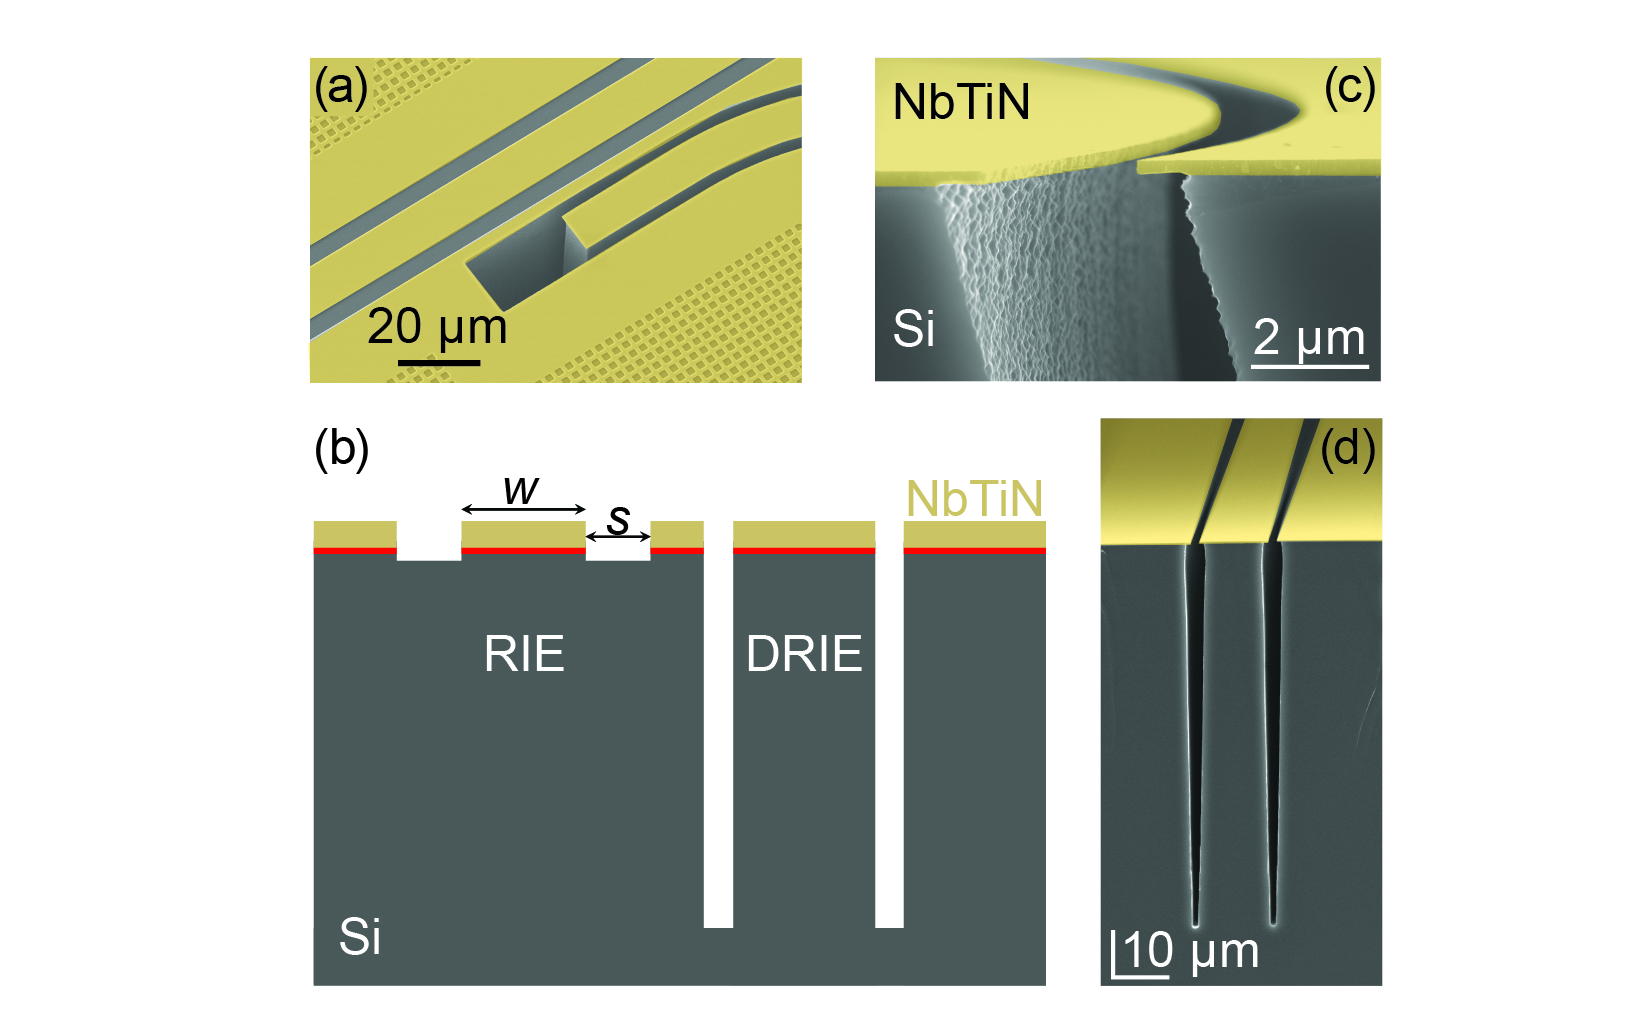
\includegraphics[width=.92\textwidth]{Figures/DRIE/DRIE figure.jpg}
    \caption{\textbf{(a)} false-colored SEM image of a RIE feedline capacitively coupled to a DRIE resonator. \textbf{(b)} Corresponding schematic cross section. The metal substrate interface treated with HMDS is shown in red. \textbf{(c)} SEM cross section of a DRIE resonator near the surface, showing the metallization (\SI{\sim300}{\nano \meter}), Si underetch (\SI{\sim1}{\micro \meter}) and sidewall roughness (\SI{\sim100}{\micro \meter}). \textbf{(d)} SEM cross section of a DRIE resonator showing that a high etch anisotropy can be obtained, with a depth of \SI{80}{\micro \meter}.}
    \label{fig:DRIE schematic}
  \end{figure}

  \subsubsection{Magnetic shielding and vortex trapping}

  % \begin{wrapfigure}[20]{r}{0.4\textwidth}
  %   \begin{center}
  %   \vspace{-30pt}
  %     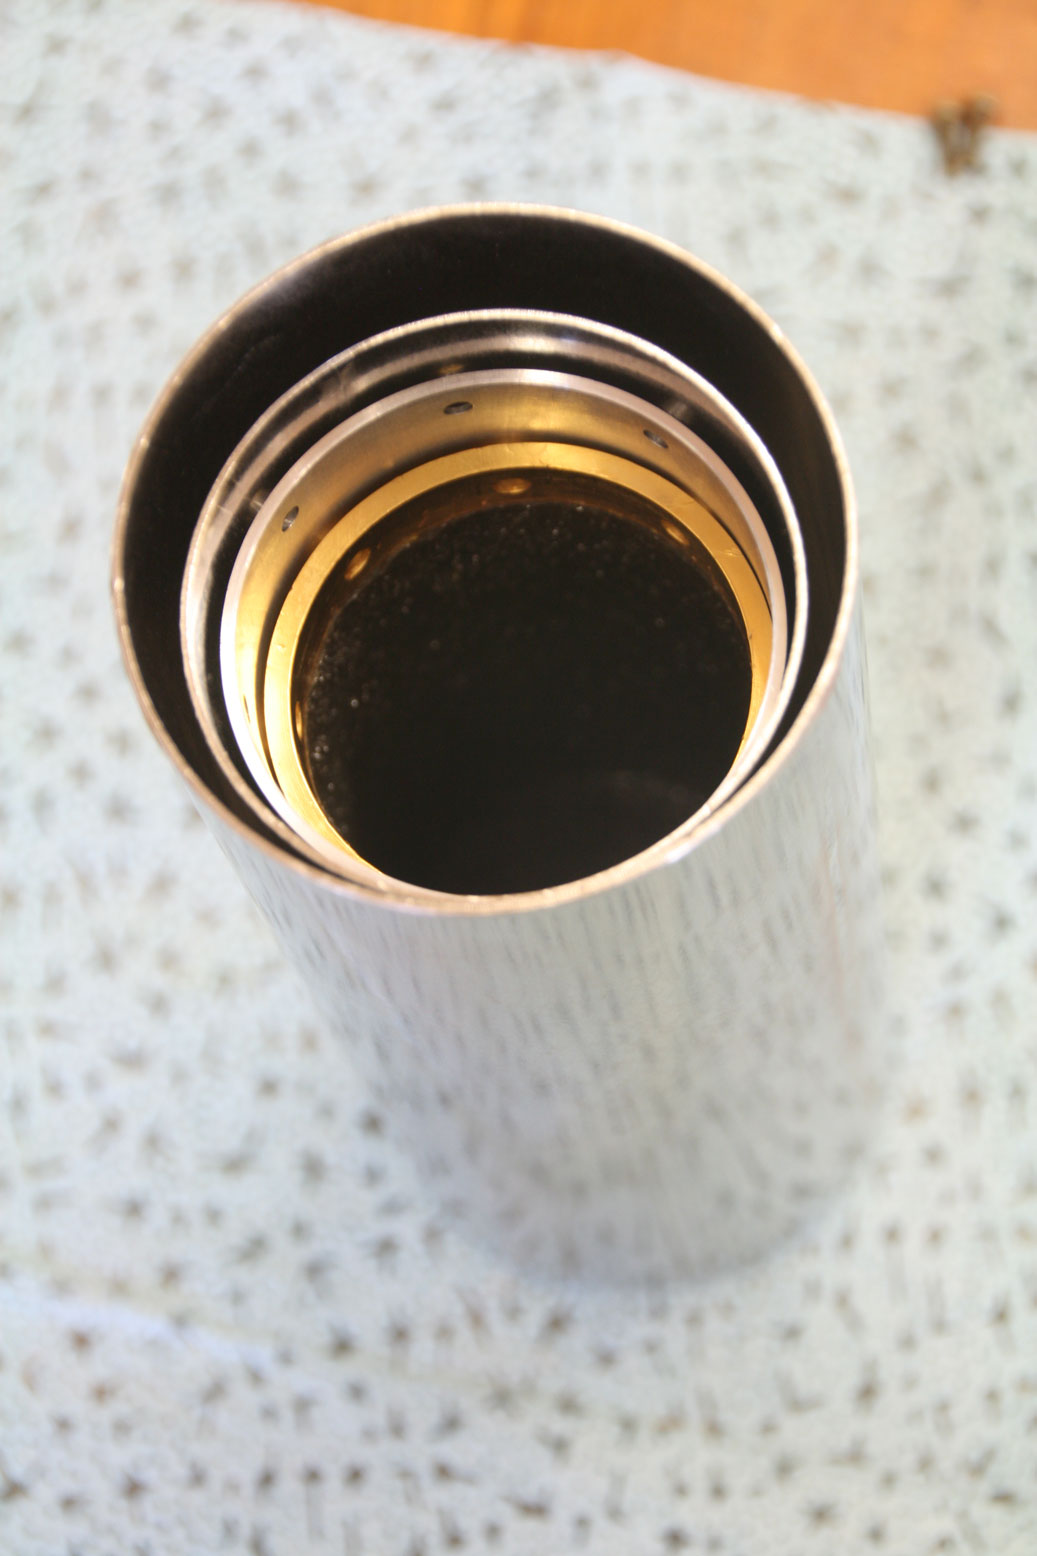
\includegraphics[width=\textwidth]{Figures/DRIE/Shielding.jpg}
  %   \end{center}
  %   \vspace{-20 pt}
  %   \caption{Different stages of shielding used. Inside the inner copper shielding is a black coating, used for IR absorption.}
  %   \label{fig:shielding}
  % \end{wrapfigure}
  Vortices are created in a superconducting thin film when a magnetic field greater than the sample-dependent threshold magnetic field is present. One method to lower the amount of vortices is to realize CPW with $w < \SIm{15}{\micro \meter}$, while using proper magnetic shielding around the sample. Furthermore, using nonmagnetic materials within the shield also results in less stray magnetic fields bring present.

  Even when using these methods to counter the presence of magnetic fields, there may still be a small amount of vortices present in the sample, which may lead to dissipation. To counter their movement a grid-like structure can be added in the superconducting material, effectively pinning the vortices.

  \begin{figure}[h]
    \centering
      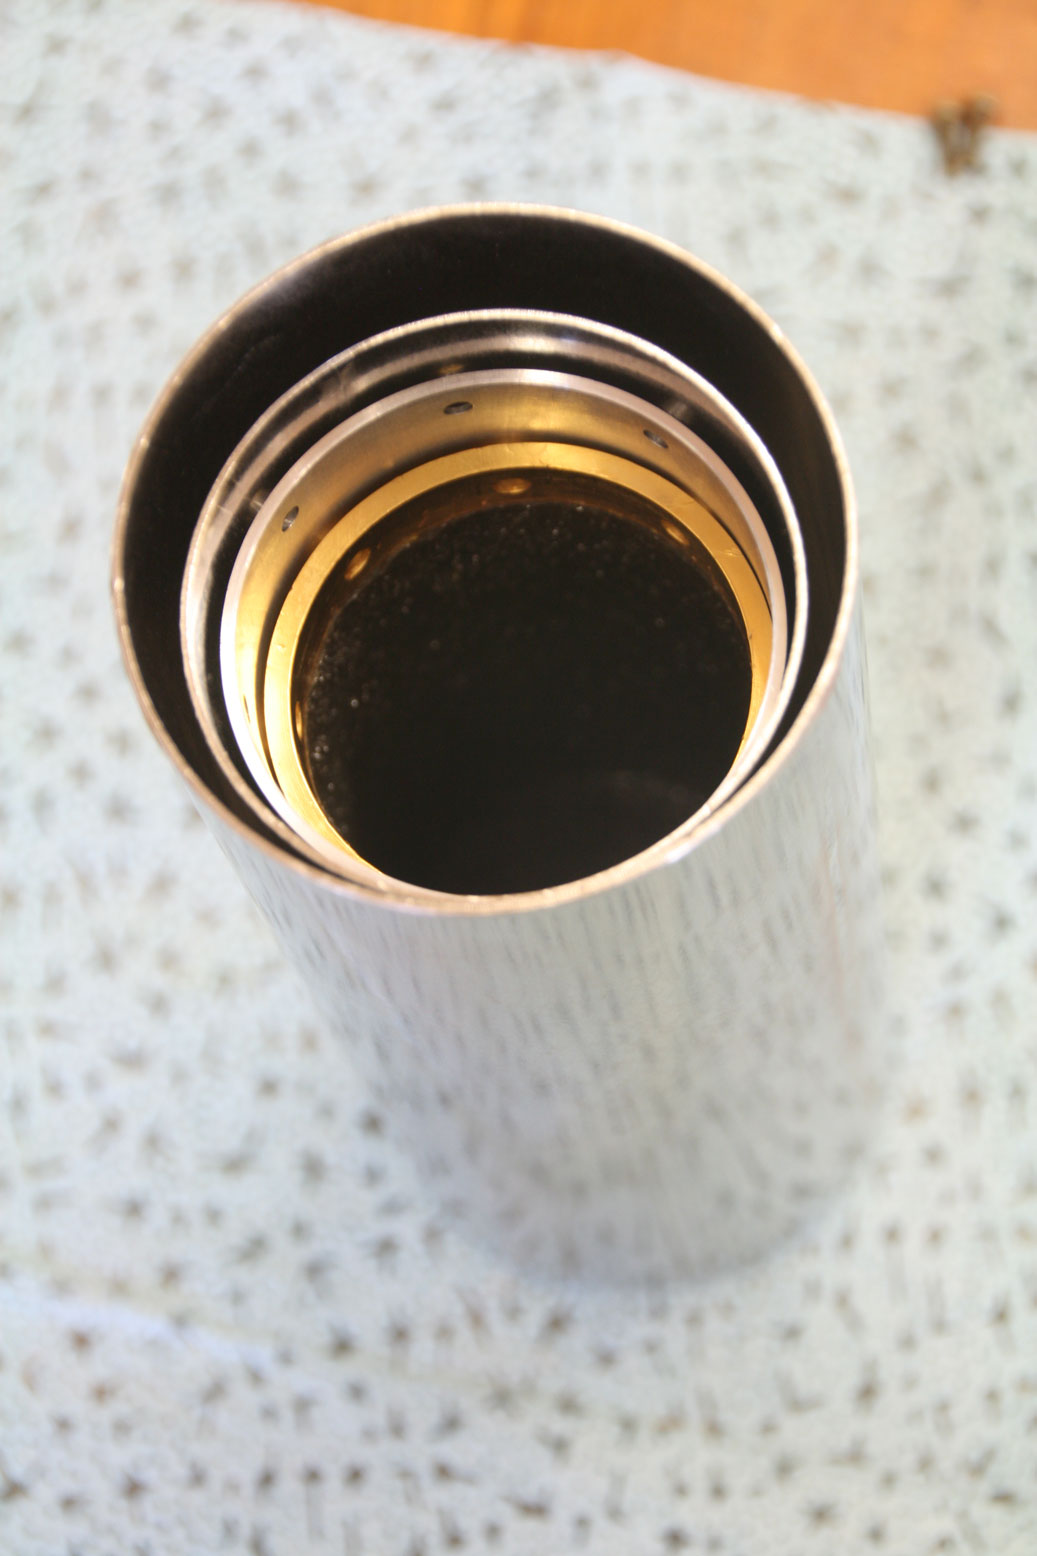
\includegraphics[width=.4\textwidth]{Figures/DRIE/Shielding.jpg}
    \caption{Different stages of shielding used. Inside the inner copper shielding is a black coating, used for IR absorption.}
    \label{fig:shielding}
  \end{figure}

\chapter{Results and discussion}
\label{ch:Results and discussion}

  \section{Experimental set-up}
    \label{sec:Experimental set-up}


    \begin{figure}[!htb]
      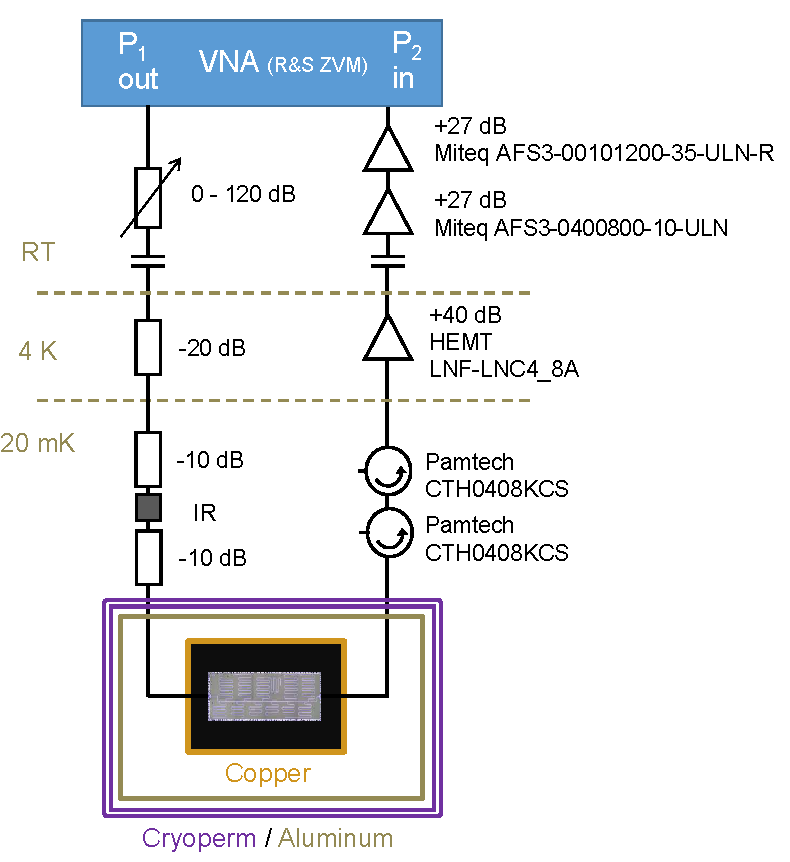
\includegraphics[width=.5\textwidth]{Figures/DRIE/FigS2_MW_setup.pdf}
      \caption[width=\textwidth]{Measurement setup used for resonator characterization in the $^{3}\mathrm{He}/^{4}\mathrm{He}$ dilution refrigerator (Leiden Cryogenics CS81): microwave schematic, magnetic shields (two Cryophy, one aluminum), IR filters (home-made Eccosorb filters), and IR adsorbers (inner surface of the inner Cu radiation shield, coated with Stycast~2850 and silicon carbide powder).}
      \label{fig:fridges}
    \end{figure}
    The experimental set-up is shown in Fig.~\ref{fig:fridges}. The fridge used in this experiment is a $^{3}\mathrm{He}/^{4}\mathrm{He}$ dilution refrigerator by Leiden Cryogenics. The refrigerator has a base temperature of \SI{\sim15}{\milli \kelvin}. Several stages of shielding are used. The sample is anchored to a copper coldfinger, directly connected to the mixing chamber of the dilution refrigerator. This is then enclosed in a copper can, the inner surface of which is coated in a mixture of Stycast 2850 and silicon carbide granules with diameters between 15 and 1000 nm to absorb IR radiation. The copper can is enclosed in a second can made from aluminum. The cans are furthermore surrounded by two layers of cryogenic magnetic shielding (1-mm-thick Cryophy, Magnetic Shields Ltd).

    The input signal is generated using a Rohde \& Schwarz ZVM vector network analyzer, connected to an Aeroflex 8310 step attenuator, which has an attenuation range of \SI{120}{\decibel}. The signal out of the fridge is measured using the same vector network analyzer.

    Using this set-up, quarter-wave resonators, fabricated by Alessandro Bruno, were measured in a frequency range between \SIrange{1}{9}{\giga \hertz}. The sample is shown in Fig.~\ref{fig:set4}. The resonators were made using NbTiN on a silicon substrate. The advantage of NbTiN is that the metal atoms are bound to nitrogen, thereby inhibiting bond formation with oxides. To minimize losses, all resonators were treated with HMDS and deep-reactive ion etching.


    Unless stated otherwise, all measurements were performed with the fridge at base temperature (\SI{\sim15}{\milli \kelvin}).

    Because the relevant regime where resonators interact with qubits is the single-photon regime, a very weak signal must must be applied to determine its properties in that regime. At these low powers noise becomes a relevant issue. In Appendix~\ref{ch:noise} the noise of the system is characterized.

    \begin{figure}[h]
      \centering
      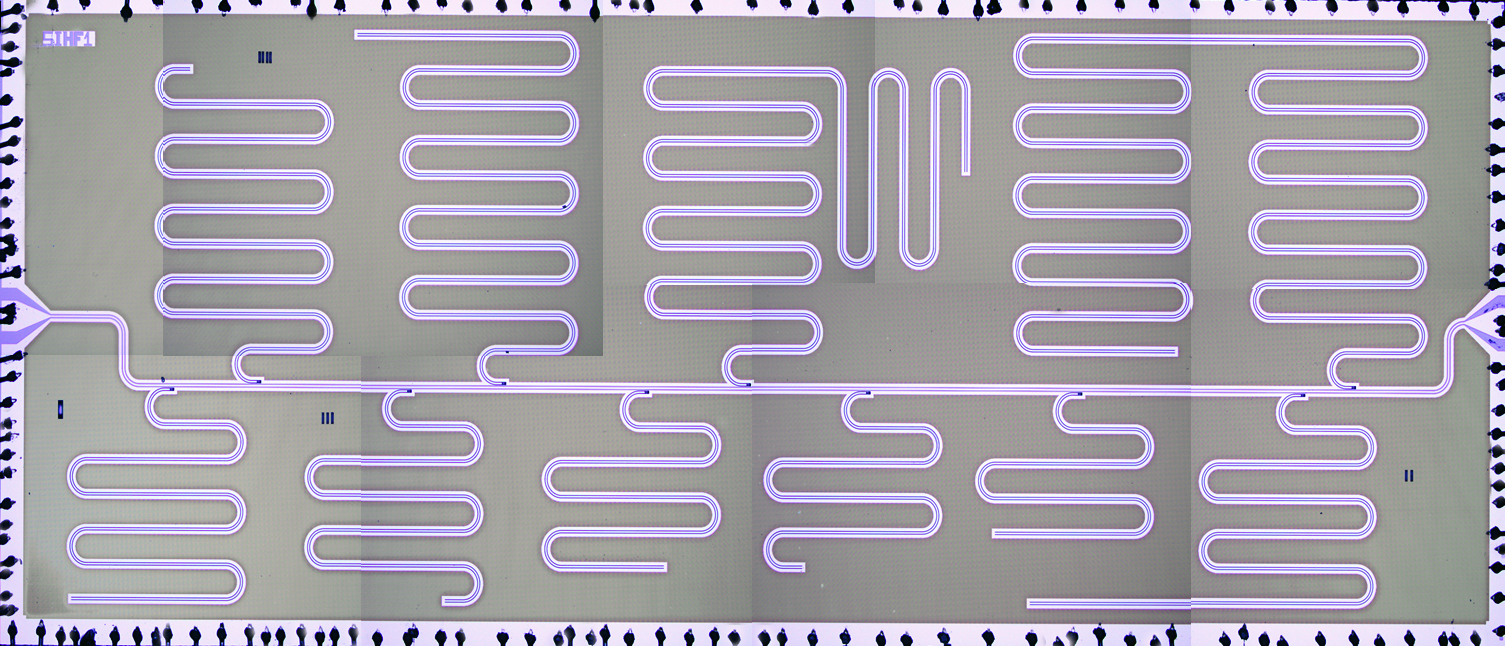
\includegraphics[width=.7\textwidth]{Figures/DRIE/All_set4.png}
      \caption{Optical microscopy image of the sample measured for the APL paper. The sample consists of ten quarter-wave resonators, with frequencies ranging between \SIrange{1}{11}{\giga \hertz}, connected to a central feedline. The resonators are made using NbTiN on a Si substrate. The sample is treated with HMDS and DRIE.}
        \label{fig:set4}
    \end{figure}



\section{Resonator measurement}

\begin{figure}[h]
    \centering
    \begin{subfigure}[b]{.49\textwidth}
        \label{fig:resonator_amplitude}
        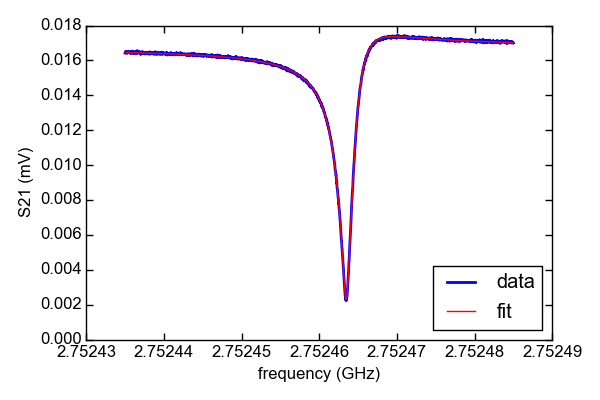
\includegraphics[width=\textwidth]{Figures/DRIE/resonator_amplitude.png}\figureinset{(a)}{2.55}{2.0}
    \end{subfigure}
    \begin{subfigure}[b]{.49\textwidth}
        \label{fig:resonator_complex}
        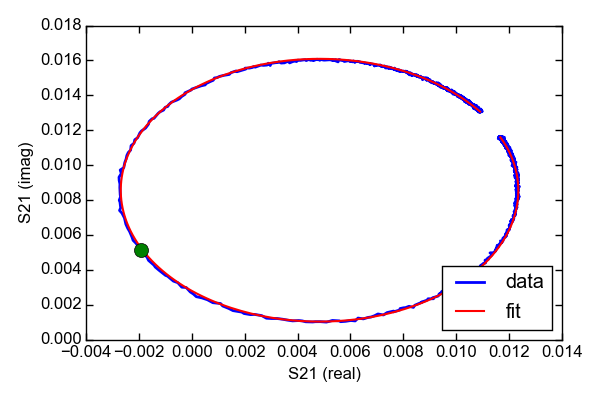
\includegraphics[width=\textwidth]{Figures/DRIE/resonator_complex.png}\figureinset{(b)}{2.55}{2.0}
    \end{subfigure}
    \caption{Forward transmission $S_{21}$ spectrum of a resonator around \SI{2.75}{\giga \hertz}. Panel (a) shows the amplitude of $S_{21}$, along with a fit (red). Panel (b) shows the path of $S_{21}$ in the complex path, along with a fit (red). The green dot indicates the resonance frequency of the resonator.  Measurement was performed at \SI{15}{\milli \kelvin} at an input power of \SI{-123}{\dBm} corresponding to $\sim 5 \times 10^4$ photons.}
    \label{fig:resonator}
\end{figure}

 At or close to the resonance frequency, the resonator will interact strongly with the feedline, resulting in a reduction in transmission (see Fig.~\ref{fig:resonator}). The corresponding frequency spectrum exhibits a Lorentzian lineshape.

  In Fig.~\ref{fig:resonator} the transmission $S_{21}$ of a resonator is shown. Figure~\ref{fig:resonator}(a) shows the transmitted voltage $|S_{21}|$ of the resonator as a function of frequency. One interesting point is that the Lorentzian exhibits an asymmetry, which is often attributed to reflections in the feedline \cite[p192]{Geerlings}. This could be caused by impedance mismatching of components in the set-up, which would result in part of the signal being reflected.

  The data has in Fig.~\ref{fig:resonator} been fitted with the following complex-valued function~\cite{bruno2015reducing}:

  \begin{equation}
    S_{21} =A \left( 1 + \alpha \frac{\omega-\omega_r}{\omega_r} \right)
    \left(1-\frac{\frac{Q_l}{\lvert Q_e \rvert}e^{i\theta}}{1+2iQ_l\frac{\omega-\omega_r}{\omega_r}}\right)e^{i\left(\phi_v f+\phi_0\right)}.
    \label{eq:THEhanger}
  \end{equation}
  Here, $\omega_r$ is the resonance frequency of the resonator, $Q_e=\left|Q_e\right|e^{i\theta}$ is the extrinsic quality factor, related to the coupling quality factor by $1/Q_c=Re\left(1/Q_e\right)$, $\alpha$ accounts for any slope in the background transmission surrounding the resonance frequency, and $\phi_v$ and $\phi_0$ account for the propagation delay to and from the sample.

\section{Power dependence}
\label{sec:resonator:results:power_dependence}

\begin{figure}
    \centering
    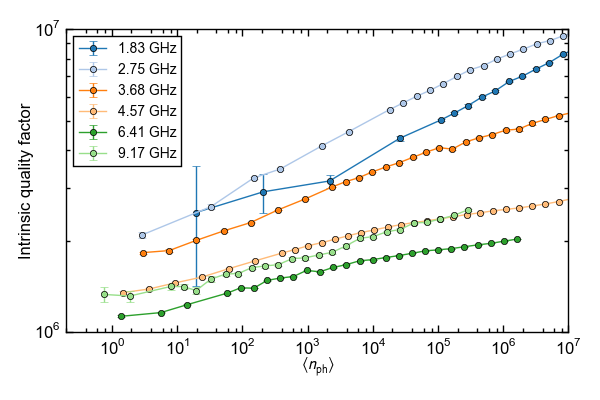
\includegraphics[width=0.8\textwidth]{Figures/DRIE/Qi_vs_n_photon.png}
    \caption{Internal quality factor of resonators as a function of mean number of photons present in the resonator. Measurements were performed at \SI{15}{\milli \kelvin}.}
    \label{fig:Qi_vs_n_photon}
\end{figure}
To be able to study the behaviour of the resonators, measurements were performed for several powers. Using proper calibrations for the attenuation down to the sample, the power can be converted to the input power at the sample. This value can then be converted to the mean number of photons present in the resonator, as described in Appendix~\ref{ch:photon number calculation}. The results are shown in Fig.~\ref{fig:Qi_vs_n_photon}.

As can be seen, all resonators measured obtain quality factors in excess of 1 million, even at the single photon regime used in quantum computation. Furthermore, the internal quality factor $Q_i$ of all resonators decrease with decreasing photon number. One explanation for this phenomenon is that the dissipation is mainly due to TLS. Since measurements were performed at \SI{\sim15}{mK}, the TLS are not saturated since the rate of thermal excitation is low. As discussed in section~\ref{sec:TLS}, the relative loss due to TLS is highest at low power, in the regime where they are not saturated. Therefore the fact that the internal quality factor $Q_i$ rises with the mean number of photons present in the resonator can be attributed to a larger amount of TLS being saturated. This would suggest that, even with HMDS and DRIE treatment of the sample, at low power and temperature, the internal quality factor is still limited by TLS being present.

As the mean photon number of a resonator is inversely proportional to the square of frequency \cite{bruno2015reducing}, for a low-frequency resonator a lower input power is required to reach the same photon population as a higher-frequency resonator. This has important consequences for the signal-to-noise ratio, and hence for the required integration time. At high photon numbers this is not a concern, as the transmitted signal is high enough to be accurately measured in a short period of time. For the single-photon powers, however, which is the region of interest for quantum computation, acquiring enough signal took up to five hours for the lowest frequencies. The reason that for the resonator with a resonance frequency at \SI{1.83}{\giga \hertz} has large error bars at low powers can be partly attributed to this, but as is seen in App.~\ref{sec:noise_results}, the main reason is that its frequency lies outside the bandwidth of the amplifiers and circulators of the set-up, resulting in a large amount of additional noise.

\section{Temperature dependence}
\label{sec:resonator:results:emperature_dependence}
\begin{figure}
    \centering
    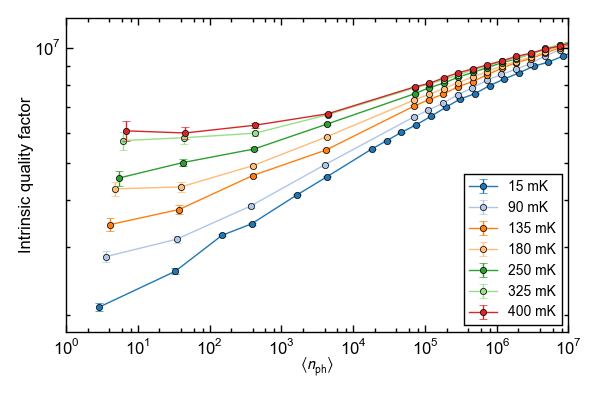
\includegraphics[width=0.8\textwidth]{Figures/DRIE/Qi_vs_n_photon_temperature_dependence.png}
    \caption{Internal quality factor versus photon number for temperatures ranging from \SI{15}{\milli \kelvin} up to \SI{400}{\milli \kelvin}. All measurements were performed for a resonator with resonance frequency $f_0 = $\SI{2.75}{\giga \hertz}.}
    \label{fig:Qi_vs_n_photon_temperature_dependence}
\end{figure}

Aside from power, some of the dissipation channels also depend on the temperature of the system. To be able to study the effect of temperature on resonators, the resonator with frequency \SI{2.75}{\giga \hertz} has been studied as a function of power for several temperatures ranging from \SI{15}{\milli \kelvin} up to \SI{400}{\milli \kelvin}. The reason for choosing this resonator is that it has the highest internal quality factor of all the resonators measured, and so any change in quality factor would be most clearly visible.

The results are shown in Fig.~\ref{fig:Qi_vs_n_photon_temperature_dependence}. As can be clearly seen, the quality factor increases with increasing temperature. This is likely due to the fact that TLS are thermally excited for a larger percentage of time. Therefore, the relative energy dissipation with respect to total energy in the resonator will be lower, resulting in an increase in quality factor.

Another interesting point is that the increase in quality factor as a function of temperature is largest at low powers. This can also be explained when the limiting factor is due to TLS. At low powers, the TLS are almost exclusively excited thermally, while at higher powers, the excitation of TLS is not only due to thermal excitations, but also from photon absorption.

If one looks at the highest temperatures, it seems that the increase in quality factor as a function of temperature seems to slowly approach a saturation point. One reason is that the TLS are approaching their saturation, and so increasing the temperature further will have little effect on the percentage of time that the TLS are in the excited state. As will be shown in the next section, at \SI{400}{\milli \kelvin} the quality factor of the resonator is close to its maximum value, and will decrease as temperature is further increased.



\section{Temperature tracking}
\label{resonator:results:temperature_tracking}
\begin{figure}[h]
    \centering
    \begin{subfigure}[b]{.49\textwidth}
        \label{fig:temperature_tracking_Qi_drop}
        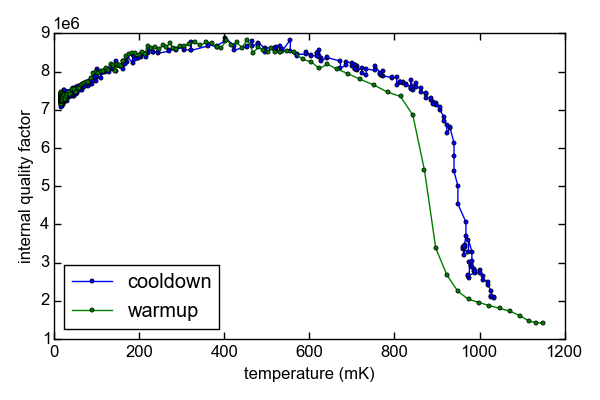
\includegraphics[width=\textwidth]{Figures/DRIE/Temperature tracking drop - Qi vs T.png}\figureinset{(a)}{2.65}{1.92}
    \end{subfigure}
    \begin{subfigure}[b]{.49\textwidth}
        \label{fig:temperature_tracking_Qi_nodrop}
        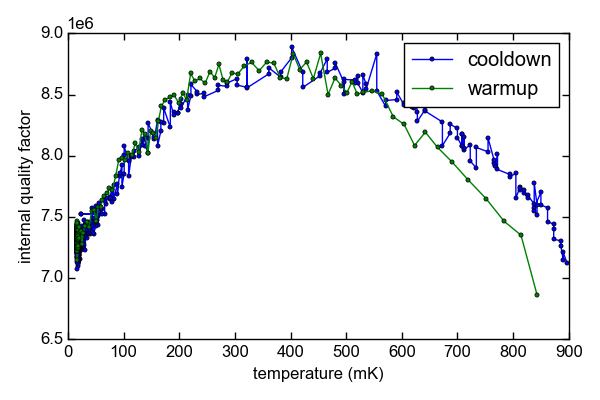
\includegraphics[width=\textwidth]{Figures/DRIE/Temperature tracking - no drop - Qi vs T.png}\figureinset{(b)}{2.57}{1.92}
    \end{subfigure}
    \caption{Internal quality factor versus temperature for the resonator with resonance frequency $f_0= $\SI{2.75}{\giga \hertz}. Quality factor was continuously measured as the sample was cooled down and warmed up four days later. Panel (a) shows the full temperature range up to the helium condensation cycle. Panel (b) shows a close-up of the region until \SI{900}{\milli \kelvin}.}
    \label{fig:temperature_tracking_Qi}
\end{figure}

To further investigate the temperature dependence of the resonator, a continuous measurement was performed on the resonator with resonance frequency \SI{2.75}{\giga \hertz} during a cool-down and a subsequent warm-up of the fridge four days later. Measurements were performed for temperatures ranging from base temperature (\SI{15}{\milli \kelvin}) to roughly \SI{1}{\kelvin}. Above this temperature, the fridge entered a cyclic helium condensation/evaporation process. All temperatures were measured at an input power of \SI{-113}{\dBm}, corresponding to roughly $5 \times 10^5$ photons. In Fig.~\ref{fig:temperature_tracking_Qi} the internal quality factor versus temperature is shown during a cooldown and subsequent warm-up of the fridge. As can be seen, the quality factor reaches a maximum quality factor at a temperature of \SI{\sim400}{\milli \kelvin}. Below this temperature, the quality factor is likely limited by the presence of TLS (see sections \ref{sec:resonator:results:power_dependence} and \ref{sec:resonator:results:emperature_dependence}). Above this temperature however, the quality factor decreases, indicating that TLS are not the limiting factor anymore for $Q_i$. One likely explanation is that the main source of dissipation is now due to the presence of quasiparticles in the resonator. At even higher powers other effects such as vortices contribute more significantly to the decay of the quality factor.

From Fig.~\ref{fig:temperature_tracking_Qi} it seems that there is some hysteresis at high temperatures. However, this is likely due to the fact that the thermometer is at a different position in the fridge as the sample, and does not thermalize equally fast. There may therefore be a delay between the temperature of the thermometer, and the actual temperature of the sample.

\begin{figure}[h!]
    \centering
    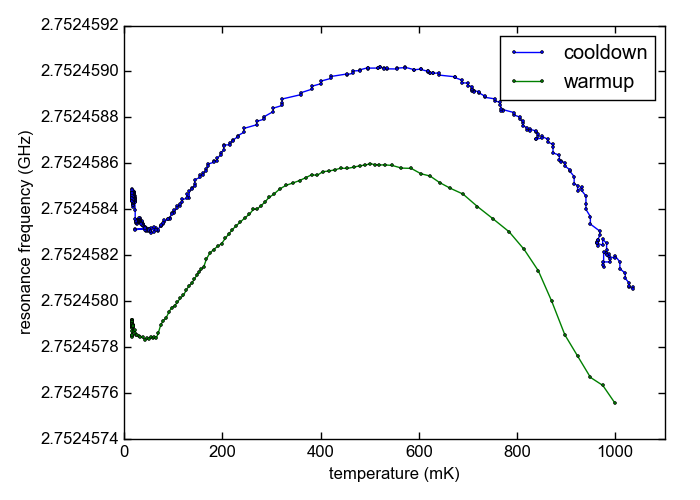
\includegraphics[width=.72\textwidth]{Figures/DRIE/Temperature tracking - f0 vs T.png}
    \caption{Resonance frequency versus temperature during a cooldown and subsequent warm-up four days later. In the period between cooldown and warm-up the resonance frequency has shifted by \SI{\sim 500}{\hertz}, possibly due to phase noise.}
    \label{fig:temperature_tracking_f0}
\end{figure}


Aside from the internal quality factor, another quantity of interest is the resonance frequency $f_0$ of the resonator, which also depends on the temperature. The result from of tracking the resonance frequency of the resonator during cooldown and subsequent warm-up is shown in Fig.~\ref{fig:temperature_tracking_f0}. As can be seen in both cases, the resonance frequency reaches a maximum around \SI{500}{\milli \kelvin}.

Between the cooldown and warm-up the resonance frequency seems to have shifted by roughly \SI{500}{Hz}. It is possible that during the four days that the sample was cooled the environment of the resonator slowly varied, which shifted the resonance frequency of the resonator. Further measurements are, however, required to determine if this is the case.

The decrease in resonance frequency at higher temperatures can be explained by the presence of quasiparticles, which increase the kinetic inductance \cite[p91]{Geerlings}. The resonance frequency is inversely proportional to the square root of the total conductance \cite{barends2008contribution}, and so an increase in kinetic inductance leads to a decrease in resonance frequency. For measurements done by Barends et al. \cite{barends2008contribution}, the change in resonance frequency due to changes in the kinetic inductance seem to roughly correspond with the decrease in center frequency measured in Fig.~\ref{fig:temperature_tracking_f0}.

\begin{figure}[h]
    \centering
    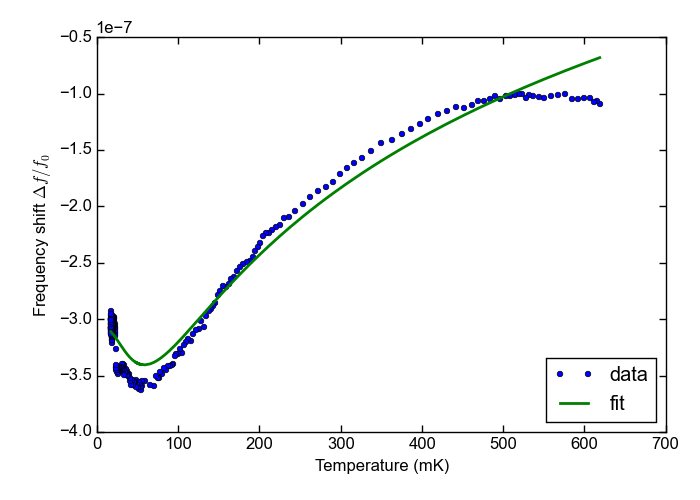
\includegraphics[width=.7\textwidth]{Figures/DRIE/Temperature increase tracking - f0 vs T with fit.png}
    \caption{Frequency shift versus temperature for low temperatures, along with fit (green). The fit was performed using the model by Gao et al.~\cite{gao2008experimental}. The fit corresponds well with data, even describing the frequency increase at the lowest temperatures.}
    \label{fig:f0_vs_T_with_fit}
\end{figure}

The decrease in resonance frequency at lower temperatures can be explained due to TLS still being present. A model is presented by Gao et al. \cite{gao2008experimental}, in which they describe the decrease in resonance frequency due to the presence of TLS. As can be seen in Fig.~\ref{fig:f0_vs_T_with_fit} the model corresponds well with the data at low temperatures. At higher temperatures the model deviates from data, which may be explained by quasiparticles dominating as source of dissipation. The model furthermore predicts an increase in resonance frequency at lowest temperatures, which Gao et al. have indeed measured~\cite{gao2008experimental}. This increase in resonance frequency can also be seen in Fig.~\ref{fig:f0_vs_T_with_fit}, further supporting the claim that at low temperatures the resonator is still limited by TLS, even after treatment of HMDS and DRIE.



\chapter{Conclusion and future work}

As we have shown, the application of HMDS surface treatment and DRIE resulted in an improvement of the internal quality factor of the resonators by almost an order of magnitude. These state of the art cQED CPW resonators all attained quality factors in excess of 1 million at single-photon level, which is the regime at which cQED circuits operate.

Since the quality factor of all resonators is found to decrease with decreasing input power, this indicates that at low temperatures and powers the limiting factor is still TLS. The fact that the quality factor initially increases with higher temperatures, supports this claim. By also measuring  the resonance frequency as a function of temperature, the curve obtained is in good agreement with a model describing the resonance-frequency shift due to TLS \cite{gao2008experimental}. The curve even shows an increase in resonance frequency at the lowest temperatures, which was also predicted by the model. These results suggest that even after HMDS surface treatment and deep-reactive ion etching was applied, the internal quality factor of the resonator at low temperatures and power is still limited by the presence of TLS. Further research needs to be done to determine at what interface the dissipation due to TLS is greatest.

The next step is to perform the same treatments (HMDS and DRIE) on transmon qubits, as it is expected that this will result in a similar increase in coherence times. This is, however beyond the task of my master thesis.
